\documentclass[border=5mm]{standalone}
\usepackage{tikz}
\usepackage{amssymb}
\usetikzlibrary{decorations.markings, arrows.meta}

\begin{document}
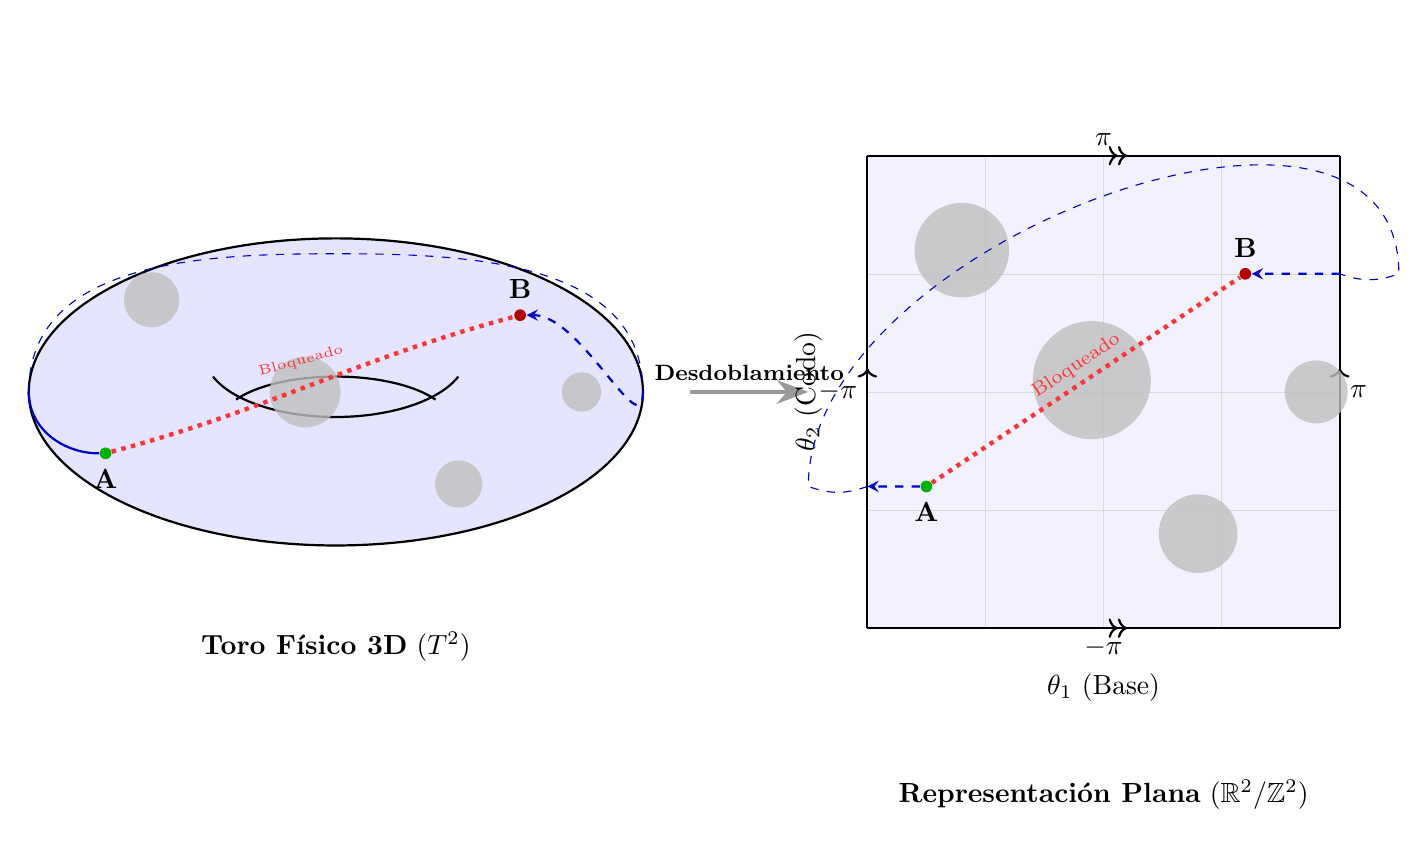
\begin{tikzpicture}[
    scale=1.5,
    % Estilo para las flechas de identificación topológica
    identify1/.style={postaction={decorate,decoration={markings,mark=at position 0.55 with {\arrow{>}}}}},
    identify2/.style={postaction={decorate,decoration={markings,mark=at position 0.55 with {\arrow{>>}}}}},
    % Estilo para los obstáculos (bolas abiertas)
    cobs/.style={circle, fill=gray!50, opacity=0.8},
    % Estilo para la trayectoria
    path/.style={thick, dashed, blue!80!black, -stealth}
]

    % ==========================================
    % PARTE IZQUIERDA: TORO 3D
    % ==========================================
    \begin{scope}[xshift=-4.5cm, yshift=0cm, scale=1.3]
        % Silueta del Toro
        \draw[thick, fill=blue!10] (0,0) ellipse (2cm and 1cm);
        
        % Agujero central
        \draw[thick] (-0.8,0.1) arc[start angle=-160, end angle=-20, x radius=0.85cm, y radius=0.4cm];
        \draw[thick] (-0.65,-0.05) arc[start angle=150, end angle=30, x radius=0.75cm, y radius=0.3cm];
        
        % Puntos A y B
        \node[circle, fill=green!70!black, inner sep=1.5pt, label=below:{\textbf{A}}] (t_a) at (-1.5, -0.4) {};
        \node[circle, fill=red!70!black, inner sep=1.5pt, label=above:{\textbf{B}}] (t_b) at (1.2, 0.5) {};

        % Obstáculos equivalentes
        \node[cobs, minimum size=0.9cm] at (-0.2, 0) {};    % Obstaculo central
        \node[cobs, minimum size=0.6cm] at (0.8, -0.6) {};  % Obstaculo inferior derecho
        \node[cobs, minimum size=0.7cm] at (-1.2, 0.6) {};  % Obstaculo superior izquierdo
        \node[cobs, minimum size=0.5cm] at (1.6, 0) {};     % Obstaculo borde derecho

        % Trayectoria directa BLOQUEADA (Roja, punteada)
        % (Parece atravesar la superficie frontal cruzando el obstáculo central)
        \draw[red!80, dotted, ultra thick] (t_a) to[out=15, in=195] (t_b);
        \node[red!80, above, rotate=15] at (-0.2, 0.1) {\tiny Bloqueado};

        % Trayectoria TOPOLÓGICA (Azul, sólida, Wrap-around)
        % (Sale de A a la izquierda, da la vuelta por atrás de la dona y llega a B)
        \draw[blue!80!black, thick] (t_a) to[out=180, in=-90] (-2, 0);
        \draw[blue!80!black, dashed] (-2, 0) to[out=90, in=180] (0, 0.9) to[out=0, in=90] (2, 0); % por atras
        \draw[path] (2, 0) to[out=-90, in=0] (t_b); % Reaparece por la derecha
        
        \node[below] at (0, -1.5) {\textbf{Toro Físico 3D} ($T^2$)};
    \end{scope}

    % Flecha de mapeo topológico
    \draw[ultra thick, -{Stealth[length=4mm]}, gray!80] (-1.5, 0) -- (-0.5, 0) node[midway, above, text=black] {\footnotesize \textbf{Desdoblamiento}};

    % ==========================================
    % PARTE DERECHA: PLANO DESDOBLADO (Unfolded)
    % ==========================================
    \begin{scope}[xshift=2cm]
        % Fondo C-space
        \fill[blue!5] (-2,-2) rectangle (2,2);
        \draw[help lines, step=1, gray!30] (-2,-2) grid (2,2);
        
        % Bordes del toro desdoblado
        \draw[thick, identify2] (-2,-2) -- (2,-2) node[midway, below] {$-\pi$};
        \draw[thick, identify2] (-2,2)  -- (2,2)  node[midway, above] {$\pi$};
        \draw[thick, identify1] (-2,-2) -- (-2,2) node[midway, left] {$-\pi$};
        \draw[thick, identify1] (2,-2)  -- (2,2)  node[midway, right] {$\pi$};

        % Ejes
        \node at (0, -2.5) {$\rotatebox{0}{$\theta_1$ (Base)}$};
        \node[rotate=90] at (-2.5, 0) {$\theta_2$ (Codo)};

        % Puntos A y B (mapeados desde el toro)
        \node[circle, fill=green!70!black, inner sep=1.5pt, label=below:\textbf{A}] (start) at (-1.5, -0.8) {};
        \node[circle, fill=red!70!black, inner sep=1.5pt, label=above:\textbf{B}] (goal) at (1.2, 1.0) {};

        % Obstáculos (Sincronizados en posición equivalente)
        \node[cobs, minimum size=1.5cm] at (-0.1, 0.1) {};   % Central
        \node[cobs, minimum size=1.0cm] at (0.8, -1.2) {};  % Inf der
        \node[cobs, minimum size=1.2cm] at (-1.2, 1.2) {};  % Sup izq
        \node[cobs, minimum size=0.8cm] at (1.8, 0) {};     % Borde derecho

        % Trayectoria directa BLOQUEADA (Roja, punteada)
        \draw[red!80, dotted, ultra thick] (start) -- (goal) node[midway, sloped, above=-1pt] {\scriptsize Bloqueado};

        % Trayectoria TOPOLÓGICA (Azul, sólida, salta la frontera izquierda-derecha)
        % Equivale a darle la vuelta a la dona
        \draw[path] (start) -- (-2, -0.8);
        \draw[path] (2, 1.0) -- (goal);
        
        % Línea representativa del salto por fuera
        \draw[blue!80!black, dashed] (-2, -0.8) to[bend left=20] (-2.5, -0.8) to[out=90, in=90] (2.5, 1.0) to[bend left=20] (2, 1.0);

        \node[below] at (0, -3.2) {\textbf{Representación Plana} ($\mathbb{R}^2/\mathbb{Z}^2$)};
    \end{scope}

\end{tikzpicture}
\end{document}
